
\chapter{\label{cha: Transformation Approach } Transformation Approach}
\section{Introduction}
We illustrate in this chapter the most important steps of our approach. Start with the first approach of transformation from omacs to pns, then the second approach to transform PNS model into XML code, ending with import the XML code, to use it in the second tools. 

\section{Transformation Approach (OMACS To PNS)\label{sec:OMACS into PNS} }% Our Work
To Transform OMACS Model into PNS Model, we start to :
\begin{enumerate}
\item Define OMACS Meta-Model 
\item Define PNS Meta-Model
\item Define the rules of Transformation
\end{enumerate}


\subsection{OMACS} 
This section describe the work on the OMACS framework, you will see the Meta-Model of OMACS in the tools and example. 
\subsubsection{Meta Model of OMACS}
\vspace{0.5cm}
To define OMACS meta model, we first load the Class Diagramm Formalism, to be able to create, manipulate our Meta-Model,
The OMACS Meta-Model contain a set of classes:
\pagebreak
\begin{itemize}
\newcommand{\localtextbulletone}{\textcolor{gray}{\raisebox{.45ex}{\rule{.6ex}{.6ex}}}}
\renewcommand{\labelitemi}{\localtextbulletone}
	\item Agent  : represent a node in the graph of MaS, and  we assign the Role for this Agent (Node) to play  
	\item Capabilities : its node in the MaS, this Entitie represent the skills Which owns by an agent
	\item Role : represented by a node in the graph, this is the work we assign for the agent 
	\item Goal : it is also a node, we assign role for an agent depending common capabilites between an agent and role in order to achieve this goal
\end{itemize}
 
\begin{figure}[th]
	\centering
 	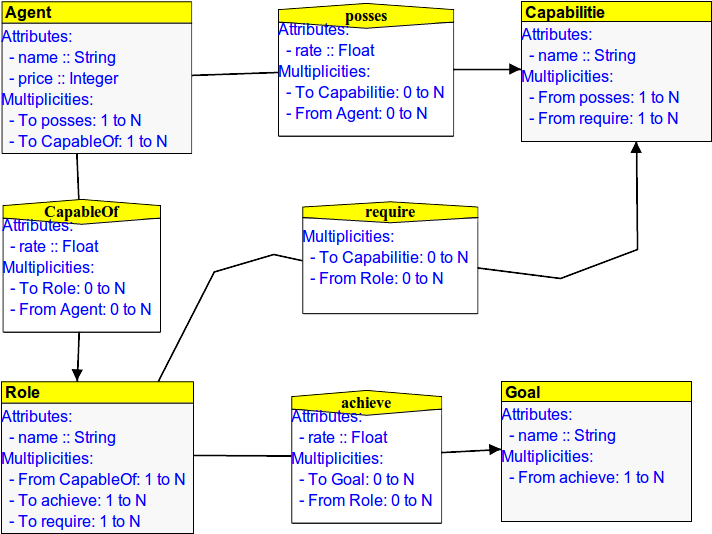
\includegraphics[scale=0.7]{ch3/img/omacs_meta}
	\caption{\label{fig:OMACS Meta-Model}OMACS Meta-Model}
\end{figure} 
\vspace{0.9cm}
figure \ref{fig:OMACS Meta-Model} illustrate OMACS Meta-Model  contain 4 classes (Agent, Capabilities, Role, Goal) 
and 4 relation (Possess, Require, CapableOf, Achieve). 
The Attribute Name in the classes represent the name of current node ,
and the rate attribute in the relation between classes represent  the relation percentage between two node or entities.

For example between an Agent and Capabilities its means how mush this Agent possese this capibilites
\pagebreak
\subsubsection{Example of OMACS}

Starting from  Meta-Model of OMACS in figure  \ref{fig:OMACS Meta-Model}, AToM3 generate a formalism of OMACS, this formalism allow us to create our OMACS Model (Multi Agent System).
\vspace{0.1cm}
\begin{figure}[th]
	\centering
 	\includegraphics[scale=0.3]{ch3/img/omacs_model}
	\caption{\label{fig:OMACS Model}Formalism of OMACS}
\end{figure} 

Example in this figure \ref{fig:OMACS Model} represent a Multi Agent system which is a contain: 2 agent and 3 Capabilities, 2 Roles, 2 Goals.
We assing 2 capabilites (C1, C2) for the Agent A1, and from other angle we se the role R1 require or demande the same capabilities the A1 has, so we can assign the R1 to A1 with the Capable of Relation, all that to achieve the Goals(G1 ,G2). 

\subsection{PNS} 

In this section we ilustrate and describe the work on the PNS framework, which is the Meta-Model of PNS in the tools and example. 
\subsubsection{Meta Model of PNS}
To define PNS meta model, we first load the Class Diagramm Formalism, and it is contain 4 classes and 4 Relation : 
\begin{itemize}

\newcommand{\localtextbulletone}{\textcolor{gray}{\raisebox{.45ex}{\rule{.6ex}{.6ex}}}}
\renewcommand{\labelitemi}{\localtextbulletone}
	\item Raw Material : its node in the graph of PNS, represent the initial material, and this node does not have any input edges 
	\item Intermediate Material : its node in the graph, represent a material in the system
	\item Final Product : it is also a node in the graph, represent the desire material 
	\item Operating Unit : it is other node type in the graph  ,represent the task or operating, it is consume the input material and produce the output material 
\end{itemize}
\pagebreak
\begin{figure}[th] 

	\centering
 	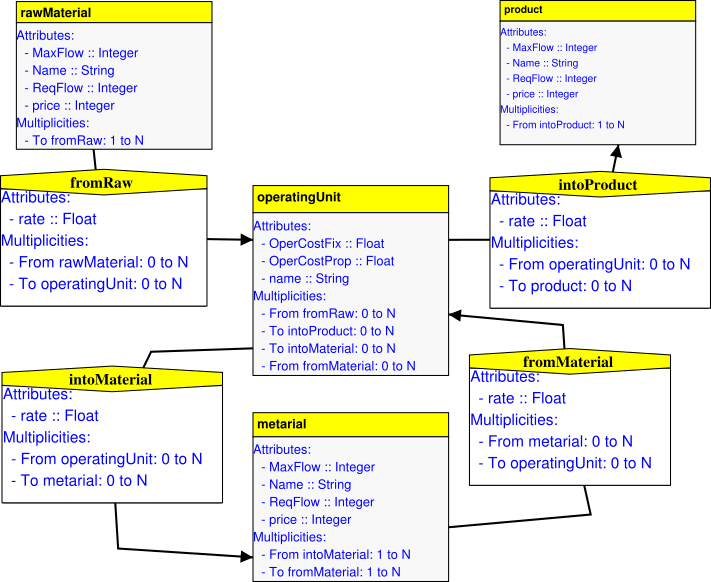
\includegraphics[scale=0.7]{ch3/img/pns_meta}
	\caption{\label{fig:PNS Meta-Model}PNS Meta-Model}
	
\end{figure} 

all material in figure \ref{fig:PNS Meta-Model} containt the same list of properties
\begin{itemize}

\newcommand{\localtextbulletone}{\textcolor{gray}{\raisebox{.45ex}{\rule{.6ex}{.6ex}}}}
\renewcommand{\labelitemi}{\localtextbulletone}

\item \textit{Name} : name of Material 
\item \textit{Price} : Price of Material
\item \textit{ReqFlow} : Requirment Flow means how much you have from this material in this system
\item \textit{MaxFlow} : Maximum Flow means how much your system can handle

\end{itemize}



and for the Operating Unit contain 3 Attribute : 
\begin{itemize}
\newcommand{\localtextbulletone}{\textcolor{gray}{\raisebox{.45ex}{\rule{.6ex}{.6ex}}}}
\renewcommand{\labelitemi}{\localtextbulletone}
\item Name : name of this Task 
\item Operating Cost Fix  : cost for entire period, Example : year
\item Operating Cost Proportional  :  cost for every Operating from this unit

\end{itemize}


\subsubsection{Example of PNS}
The AToM3 Tools  generate a formalism from the meta model we created before, load it and use it like figure \ref{fig:PNS Model} 

\begin{figure}[th]
	\centering
 	\includegraphics[scale=0.3]{ch3/img/pns_model}
	\caption{\label{fig:PNS Model}Formalism of PNS}
\end{figure} 

the figure \ref{fig:PNS Model} represent system de production contain 2 raw material and one intermediate material, final product and 3 operating unit.





\pagebreak
\subsection{Graph Grammar}
A Graph grammar is a grammar consisting of a set of rules, allow to 
Transform a formalisms of the same nature or of a different nature. 

Each Rule is composed of two parts, the left part (LHS) and the right part (RHS).
Each part can be a subgraph of the formalisms considered in the transformation

in our work, the formalisms considered in the transformation are formalism
OMACS as source graph to be transformed to PNS as target graph.

This grammar is defined bu using the tool AToM3 according to the following step

\begin{enumerate}
	\item Load OMACS and PNS meta-models
	\item Create the transformation grammar
	\item Define the rules of grammar
	\item Generate the executable file of the grammar
\end{enumerate}

Our grammar is composed of :
\begin{description}
	\item [{Rules :}]  each rule is characterized
	by a name and execution priority. They are classified in 04 categories :
\end{description}


\paragraph{\emph{1)~Collect Categorie :} } 
Rules for Collecting and create relation between some entitie.
 
\paragraph{\emph{2)~Transform Categorie:} } 
Rules for transforming nodes or links into materials or operating units.
 

\paragraph{\emph{3)~Links Categorie:} } 
Rules to links generated materials and operating units.

\paragraph{\emph{4)~Cleaning Categorie:} } 
Rules to cleaning unnecessary entities from the result .


Our approach contain 20 rules, we quote the most important transformation rules into the following steps  : 

Will notice these words in LHS(ANY \footnote{ANY:its attribue in the node and the engine will select every node with ANY attribute value} ) and RHS(COPIED\footnote{COPIED:copie the attribue value from the node with same GGLabel in LHS} , SPECIFIED \footnote{SPECIFIED:specified the attribue value manualy or by python code})
 

\paragraph{\emph{1)~Agent2RoleLink1 : Create the direct link  between the Agent and the Role (order 1) :} } The Figure \ref{fig:Create link between Agent and Role} illustrate how to create link between the agent and role depending on commun capabilities, order 1 mean it is the first rule applied in the grammar. 

\vspace{1cm}
\begin{figure}[th]
\centering
	\subfloat[LHS]{\includegraphics[scale=0.9]{ch3/img/L1}}
		\quad{}
		
\includegraphics{ch3/img/sep}
		\quad{}
	\subfloat[RHS]{\includegraphics[scale=0.9]{ch3/img/R1}}
\caption{\label{fig:Create link between Agent and Role}Assign Role to Agent } 
\end{figure}
 

\paragraph{\emph{1.1)~Condition for the rule Assign Role to Agent  :  } } 
 
Test if there is a node agent, role visited before 
in order not to fall in infinity loop, figure \ref{fig:Create link between Agent and Role} represent the rule.
 
\begin{figure}[th]
	\centering
 	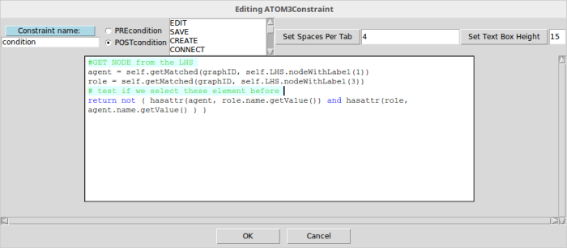
\includegraphics[scale=0.37]{ch3/img/condrule1}
	\caption{\label{fig:Condition link agent with role}Condition link agent with role  }
\end{figure} 

\paragraph{\emph{2)~ TransAgent2Raw : Transform Agent to Raw Material (order 9) :} }
Application of this rule in (figure \ref{fig:Generate for each agent raw material}) makes it possible to transform  every Agent in Multi Agent System into raw material, it has the same name and price.
\vspace{1cm} 
\begin{figure}[th]
\centering
	\subfloat[LHS]{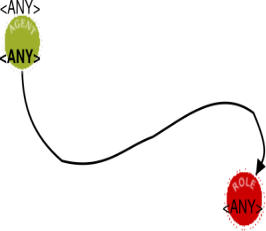
\includegraphics[scale=0.9]{ch3/img/L2}}
	\quad{}
		
\includegraphics{ch3/img/sep}
	\quad{}
	\subfloat[RHS]{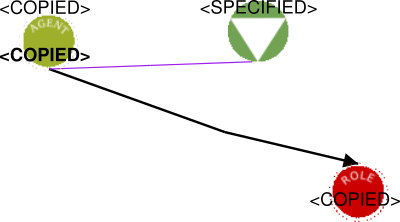
\includegraphics[scale=0.9]{ch3/img/R2}}
\caption{\label{fig:Generate for each agent raw material}Transform Agent to Raw-material} 
\end{figure}
\vspace{1cm}

%% ------------------------------------------------------------------------------------------------ order 7 
\paragraph{\emph{3)~ TransLinkAR2OpUnit : Transform Link between Agent and Role into Operating Unit (order 10) :} } This rule (Figure \ref{fig:Operating Unit for every link capable of playing}) allow to transform, the relation capable of playing between an agent and role  into operating unit.
\vspace{1cm}
\begin{figure}[th]
	\centering
	\subfloat[LHS]{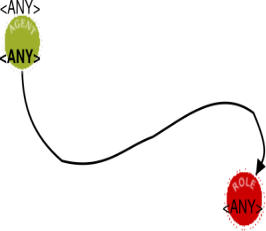
\includegraphics[scale=0.9]{ch3/img/L3}}
	\quad{}
		
\includegraphics{ch3/img/sep}
	\quad{}
	\subfloat[RHS]{\includegraphics[scale=0.9]{ch3/img/R3}}
\caption{\label{fig:Operating Unit for every link capable of playing}Transform CapableOf relation into operating unit} 
\end{figure}
\pagebreak

%% ------------------------------------------------------------------------------------------------ order 9 
\paragraph{\emph{4)~ TransGoal2Mat : Transform Goal to intermediate material (order11):} }
Application of the rule illustrated in (Figure \ref{fig:Transform Goal to intermediate material}) Transform a goal in MaS into intermediate material in process system.
 
\begin{figure}[th]
\centering 
	\subfloat[LHS]{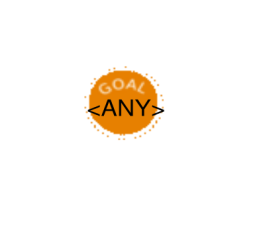
\includegraphics[scale=0.9]{ch3/img/L4}}
	\quad{}
		
\includegraphics{ch3/img/sep}
	\quad{}
	\subfloat[RHS]{\includegraphics[scale=0.9]{ch3/img/R4}}
\caption{\label{fig:Transform Goal to intermediate material}Transform Goal to intermediate material}
 
\end{figure} 
\vspace{1cm}
%% ------------------------------------------------------------------------------------------------ order 10 
\paragraph{\emph{5)~ CreateFinalStat : Create the Product node (order 13) :} }
Create the final material stat in the system. If you notice the LHS is empty because this rule applied for one time, and this rule represented in 
(Figure \ref{fig:Create the final material} ).
 
\begin{figure}[th]
\centering
	\subfloat[LHS]{
\includegraphics[scale=1.2]{ch3/img/empty_LHS}}% l5
	\quad{}
		
\includegraphics{ch3/img/sep}
	\quad{}
	\subfloat[RHS]{
\includegraphics[scale=0.9]{ch3/img/R5}}
\caption{\label{fig:Create the final material}Create the final material}
 
\end{figure} 
\pagebreak
\paragraph{\emph{5.1)~Condition for Create Final Stat : } } 
This conditon test if this attribute Final stat equal zero 
, in other word we did not visite this rule before, the rule in figure\ref{fig:Create the final material}.
 \vspace{1cm} 
\begin{figure}[th]
	\centering
 	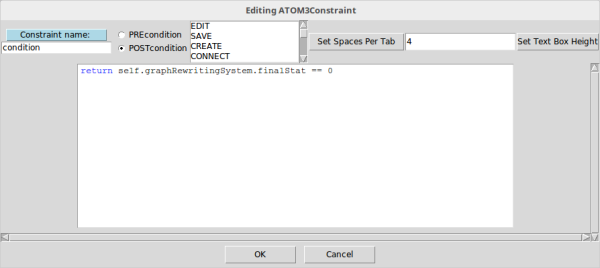
\includegraphics[scale=0.37]{ch3/img/condfinal}
	\caption{\label{fig:Condition of generate final stat } Condition of generate final stat }
\end{figure} 

%% ------------------------------------------------------------------------------------------------ order  13
\paragraph{\emph{6)~ CreateMatARG : Generate auxiliary part  (order 14) :} }

The Application of this rule generate the auxiliary part which is intermediate material consumed by operating unit, and the auxiliary part represent an agent capable to play a role in order to achieve a specific goal (Figure \ref{fig:Generate auxiliary part}).
\vspace{1cm}
\begin{figure}[th]
\centering 
	\subfloat[LHS]{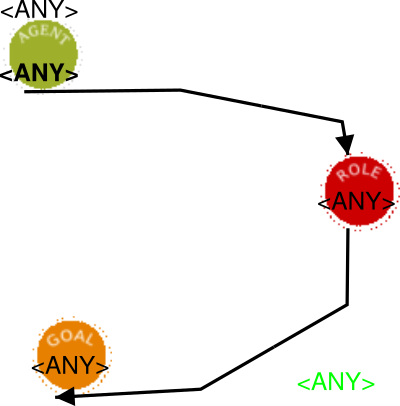
\includegraphics[scale=0.9]{ch3/img/L6}}
	\quad{}
		
\includegraphics{ch3/img/sep}
	\quad{}
	\subfloat[RHS]{\includegraphics[scale=0.9]{ch3/img/R6}}
\caption{\label{fig:Generate auxiliary part} Generate auxiliary part}
\end{figure}
\pagebreak


%% ------------------------------------------------------------------------------------------------ order  15
\paragraph{\emph{7)~ CreateLinkMatr2OAF : Create Operating unit between goal material and the product (order 15) :} }
 
 
The rule (Figure \ref{fig:Create Operating unit between  goal and OAF}) 
create an operating unit  between the final material and the goals material.
  
\vspace{1cm}
\begin{figure}[th]
\centering 
	\subfloat[LHS]{\includegraphics[scale=0.9]{ch3/img/L7}}
	\quad{}
		
\includegraphics{ch3/img/sep}
	\quad{}
	\subfloat[RHS]{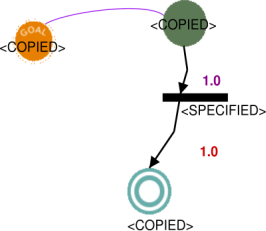
\includegraphics[scale=0.9]{ch3/img/R7}}
\caption{\label{fig:Create Operating unit between  goal and OAF}Create Operating unit between  goal and OAF}
 
\end{figure}
\vspace{1cm}


%% ------------------------------------------------------------------------------------------------ order  19
\paragraph{\emph{8)~ CreateLinkMat-ARG2Goal : Create link between auxiliary part and  goal material  (order 19) :} }
 
 
The rule in (Figure \ref{fig:link between auxiliary part and goal})  describe 
how to link the auxiliary part with right goal.  
\vspace{1cm}
\begin{figure}[th]
\centering

	\subfloat[LHS]{\includegraphics[scale=2.2]{ch3/img/L8}}
	\quad{}\quad{}
		
\includegraphics{ch3/img/sep}
	\quad{}\quad{}
	\subfloat[LHS]{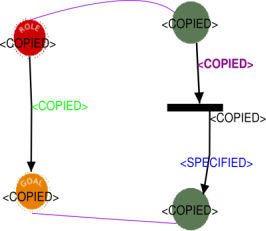
\includegraphics[scale=2.2]{ch3/img/R8}}
  
\caption{\label{fig:link between auxiliary part and goal}link between auxiliary part and goal}
 
\end{figure}
\pagebreak
\paragraph{\emph{8.1)~Condition for rule link between AUX part and Material Goal } : }
Here we check if we did not visited before  and the name of Auxiliary Part end with goal name to link it with the right goal material, the rule in figure \ref{fig:link between auxiliary part and goal}.
 
\vspace{1cm}
 
\begin{figure}[th]
	\centering
 	\includegraphics[scale=0.37]{ch3/img/condaux}
	\caption{\label{fig:Condition of Auxiliary part}Condition of Auxiliary part  }
\end{figure} 


%% ------------------------------------------------------------------------------------------------ order  20
\paragraph{\emph{9)~ CreatLinkRaw2AR : Create link to consume the raw material by operating unit  (order 20) :} }
 
 
This Figure \ref{fig:consume the raw material by operating unit}  illustrate  this rule, and it about how to create an arc between 
the raw material was generated from an agent and the operating unit.

\begin{figure}[th]
\centering
 	\subfloat[LHS]{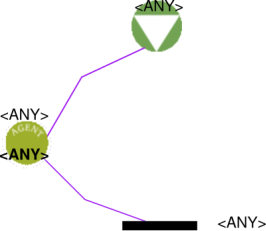
\includegraphics[scale=2.9]{ch3/img/L9}}
		\quad{}\quad{}
			
\includegraphics{ch3/img/sep}
	\quad{}\quad{}
	\subfloat[LHS]{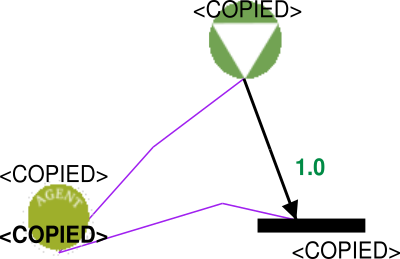
\includegraphics[scale=2.2]{ch3/img/R9}}
\caption{\label{fig:consume the raw material by operating unit} consume the raw material by operating unit}
\end{figure}




\subsection{Examples }

\subsubsection{Simple multi Agent System }
This example represents a very simple system composed of  two agent and 3 capabilities, 2 role and 2 goals.
 Figure \ref{fig:Example 1 Multi Agent System } illustrates this example :
\begin{figure}[th]
	\centering
 	\includegraphics[scale=0.3]{ch3/img/omacs_model}
	\caption{\label{fig:Example 1 Multi Agent System }Example 1 Multi Agent System}
\end{figure} 

The purpose of this example is to demonstrate the transformation of multi agent system represented in OMACS into pns model

Figure \ref{fig:Multi Agent System After transformation } shows the transformation result.
It is clear that the resulting contain a set of material and operating unit
 
\begin{itemize}

\newcommand{\localtextbulletone}{\textcolor{gray}{\raisebox{.45ex}{\rule{.6ex}{.6ex}}}}
\renewcommand{\labelitemi}{\localtextbulletone}
\item The raw material A1, A2 represent the agent  
\item The operating unit A1 R1 represent the relation between an A1 and R1 
in Mas before the transformation its the same for other entities like this one
\item the operating unit and material named A2 R2 G2 represent agent A2 Playing R2 in order to achieve G2, it is the same for other entities  

\item the operating unit and material named A2 R2 G2 represent agent A2 Playing R2 in order to achieve G2 
\end{itemize}
  
\begin{figure}[th]
	\centering
 	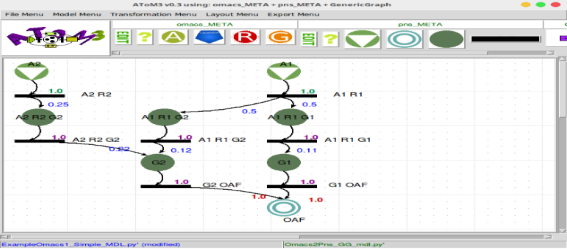
\includegraphics[scale=0.3]{ch3/img/ex1pns}
	\caption{\label{fig:Multi Agent System After transformation }Multi Agent System After transformation}
\end{figure}  
\subsubsection{ Complex multi Agent System }
This example represents a complex system composed of  3 agent and 4 capabilities, 2 role and 4 goals. Figure \ref{fig:Example 1 Multi Agent System } illustrates this example ,
 


\begin{figure}[th]
	\centering
 	\includegraphics[scale=0.3]{ch3/img/article}
	\caption{\label{fig:Complex Multi Agent System}Complex Multi Agent System}
\end{figure} 

\begin{itemize}

\newcommand{\localtextbulletone}{\textcolor{gray}{\raisebox{.45ex}{\rule{.6ex}{.6ex}}}}
\renewcommand{\labelitemi}{\localtextbulletone}
	\item every agent possesses a set of capabilites. For example A1 possese all capabilies in the system
	\item Role require a list of capabilies every agent has the same capabilies or more, so he can play this role 
	\item the Agent A1 possesses all capabilites in the system so we can say, A1 capable of playing R1 and R2
	\item Agent A1 capable of playing all roles in this system, so he can achieve all goal in the system
\end{itemize}
\vspace{0.7cm}
after the Transformation of Multi agent system from OMACS framework into PNS framework, we obtain the model is represented in figure \ref{fig:Complex Multi Agent System After transforamtion} 
and next table represent the value of the edges this model 

 % Please add the following required packages to your document preamble:
% \usepackage{booktabs}

\begin{table}[h!]
\centering
\begin{tabular}{@{}ccc@{}}
\toprule
\textbf{Operating Unit} & \textbf{Input Material} & \textbf{Output Material}                                                                              \\ \midrule
G1OAF                   & G1(1)                   & OAF (1)                                                                                               \\
G2OAF                   & G2(1)                   & OAF(1)                                                                                                \\
G3OAF                   & G3(1)                   & OAF(1)                                                                                                \\
G4OAF                   & G4(1)                   & OAF(1)                                                                                                \\ \midrule
A1R1G1                  & A1R1G1(0.433)           & G1(0.2)                                                                                               \\
A1R1G2                  & A1R1G2(0.433)           & G2(0.4)                                                                                               \\
A1R1G3                  & A1R1G3(0.433)           & G3(0.6)                                                                                               \\
A1R1G4                  & A1R1G4(0.433)           & G4(0.8)                                                                                               \\
A1R2G1                  & A1R2G1(0.433)           & G1(1.0)                                                                                               \\
A1R2G2                  & A1R2G2(0.433)           & G2(0.7)                                                                                               \\
A1R2G3                  & A1R2G3(0.433)           & G3(0.4)                                                                                               \\
A1R2G4                  & A1R2G4(0.433)           & G4(0.1)                                                                                               \\
A2R2G1                  & A2R2G1(0.633)           & G1(1.0)                                                                                               \\
A2R2G2                  & A2R2G2(0.633)           & G2(0.7)                                                                                               \\
A2R2G3                  & A2R2G3(0.633)           & G3(0.4)                                                                                               \\
A2R2G4                  & A2R2G4(0.633)           & G4(0.1)                                                                                               \\
A3R2G1                  & A3R2G1(0.5)             & G1(1.0)                                                                                               \\
A3R2G2                  & A3R2G2(0.5)             & G2(0.7)                                                                                               \\
A3R2G3                  & A3R2G3(0.5)             & G3(0.4)                                                                                               \\
A3R2G4                  & A3R2G4(0.5)             & G4(0.1)                                                                                               \\ \midrule
A1R1                    & A1                      & \begin{tabular}[c]{@{}c@{}}A1R1G1(0.433) ,A1R1G2(0.433) \\ ,A1R1G3(0.433) ,A1R1G4(0.433)\end{tabular} \\ \midrule
A1R2                    & A1                      & \begin{tabular}[c]{@{}c@{}}A1R2G1(0.433) ,A1R2G2(0.433) ,\\ A1R2G3(0.433) ,A1R2G4(0.433)\end{tabular} \\ \midrule
A2R2                    & A2                      & \begin{tabular}[c]{@{}c@{}}A2R2G1(0.633) ,A2R2G2(0.633) ,\\ A2R2G3(0.633) ,A2R2G4(0.633)\end{tabular} \\ \midrule
A3R2                    & A3                      & \begin{tabular}[c]{@{}c@{}}A3R2G1(0.5) ,A3R2G2(0.5) ,\\ A3R2G3(0.5) ,A3R2G4(0.5)\end{tabular}         \\ \bottomrule
\end{tabular}

\caption{Value of PNS Model}
\label{Value of PNS Model}
\end{table}


% Add table HEre
 \begin{landscape}
\begin{figure}[th]
	\centering 
 	\includegraphics[scale=1.3]{ch3/img/articlePNS2}
	\caption{\label{fig:Complex Multi Agent System After transforamtion}Complex Multi Agent System After transforamtion}
\end{figure} 
 
 \end{landscape}


% now we have the MaS in PNS Form 
% and there Tools called PGraphStudio
%
%
\section{Transformation Approach (PNS To XML file)\label{sec:xml} }
In Section \ref{sec:OMACS into PNS} we presented our transformation approach That allows 
to transform the OMACS to PNS.

The purpose of this transformation is the Optimization and for this we
Proposed Another processing approach That transforms PNS to XML 
files, to find the optimum structure.
\subsection{ Graph Grammar }
this grammar is Composed of three parts: 
before we start, i want to description the most important tags in this xml format :
\begin{itemize}

\newcommand{\localtextbulletone}{\textcolor{gray}{\raisebox{.45ex}{\rule{.6ex}{.6ex}}}}
\renewcommand{\labelitemi}{\localtextbulletone}
\item PGraph : this is the root tag contain all the next tags
\item Materials : This tag contain all the material tags from any kind (raw, intermediate, final)
\item OperatingUnits : This tag contain all Operating units
\item Edges : contain all edges between all nodes in the graph
\end{itemize} 

\begin{itemize}
\item \textbf{Initial Action : } This portion of our grammar is used to initialize all
Global variables used. They are used to meet various needs.  in Figure \ref{fig:Code Initial Action} 

\end{itemize}

\begin{figure}[th]
	\centering  %[scale=1.2]
 	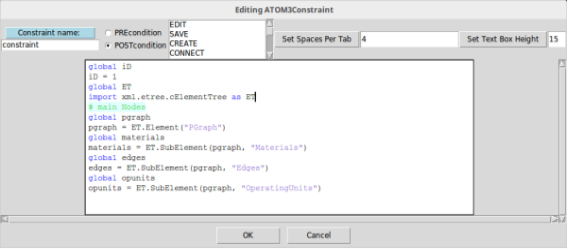
\includegraphics[scale=0.38]{ch3/img/InitAct}
	\caption{\label{fig:Code Initial Action}Code Initial Action}
\end{figure} 


\pagebreak
\begin{itemize}
\item \textbf{ Set of Rules : } 
 
Our grammar graphs Consists of ten rules. Each
rule is Characterized by a name and an execution priority. 

\end{itemize}
We cite here The Most important rules: 
\paragraph{\emph{1)~Transform RawMaterial into XML code :} }
This rule (Figure \ref{fig:Raw Material into Xml}) it is the first rule applied on the Model. To transforms the place to a XML
tags.
\begin{figure}[th]
\centering

\subfloat[LHS]{\includegraphics[scale=0.5]{ch3/img/xL1}}
\quad{}

\includegraphics{ch3/img/sep}
\quad{}
\subfloat[RHS]{
\includegraphics[scale=0.5]{ch3/img/xR1}}
 
 
\caption{\label{fig:Raw Material into Xml}Raw Material into Xml} 

\end{figure} 

\paragraph{\emph{ a )~Condition for Raw To Xml  } } For the application of this rule, it must be verified that the partition To be transformed is not treated before
\vspace{1cm}
\begin{figure}[th]
	\centering  %[scale=1.2]
 	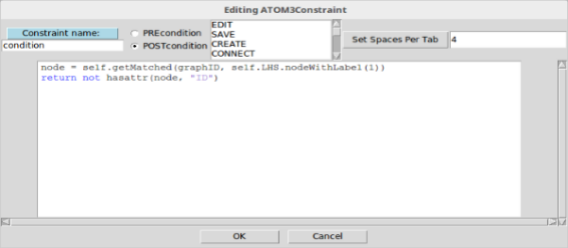
\includegraphics[scale=0.38]{ch3/img/xcond1}
	\caption{\label{fig:condition of Raw Material for Transfromation}condition of Raw Material for Transfromation}
\end{figure}
\pagebreak
\paragraph{\emph{ b )~Action for rule \ref{fig:Raw Material into Xml} } }  Once 
The rule is applied, its Action Allows to create a XML code and mark the object from the left side to processed.  
 
\begin{figure}[th]
	\centering  %[scale=1.2]
 	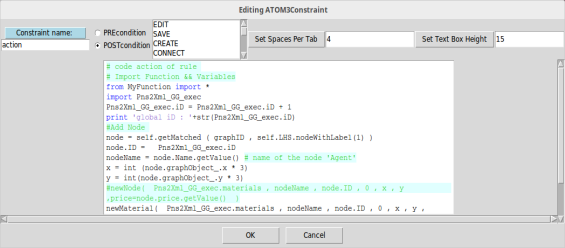
\includegraphics[scale=0.38]{ch3/img/xact1}
	\caption{\label{fig:Action of Raw Material for Transfromation}Action of Raw Material for Transfromation}
\end{figure}  
First line we import MyFunction is external file, Python code 
to be easy to manipulate  and this is the function to add new material (raw ,
intermadiate, final ) 
and for the operating unit is the same function
 
\begin{lstlisting}[language=Python, caption=Python Function Material]
def newMaterial(  parent=None, name= "None", ID="0", Type= "None", xN ='-1', yN ='-1' ,price='-1' ,reqF = 0  ,maxF =999999 ):
	#Create new Node has the Material Name...and add it into the parent node
	node = ET.SubElement(parent, "Material",ID=str(ID),Name=name,Type=str(Type))
    print 'add Cords into node		-NewNode-'
	#Create Corde for the node material
	cords = ET.SubElement(node, "Coords")
	ET.SubElement(cords, "X").text = str( xN )
	ET.SubElement(cords, "Y").text = str( yN )
	#Test if the patameter is not null or empty
	if price != '-1' or  reqF != 0  or maxF !=999999 : 
		ParameterList = ET.SubElement(node, "ParameterList")
		ET.SubElement(ParameterList, "Parameter",Name="price",Value=str( price) )
		if reqF == 0 : reqF = '-1'
		ET.SubElement(ParameterList, "Parameter",Name="reqflow",Value= str(reqF) )
		if maxF == 999999 : maxF = '-1'
		ET.SubElement(ParameterList, "Parameter",Name="maxflow",Value=str(maxF) )
	#Create Label for the MaterialNode
	label = ET.SubElement(node, "Label",Text = str(name))
	offset = ET.SubElement(label,  "Offset")
	ET.SubElement(offset, "X").text =   str(5)
	ET.SubElement(offset, "Y").text =   str(0)
	return node
\end{lstlisting}

\paragraph{\emph{2)~Transform Edge between two entitie into XML code :} } in this transformation 
we want to create link between nodes Material and Operating unit 
and we have  4 type of Edges : 
\begin{itemize}

\newcommand{\localtextbulletone}{\textcolor{gray}{\raisebox{.45ex}{\rule{.6ex}{.6ex}}}}
\renewcommand{\labelitemi}{\localtextbulletone}
	\item Edges from raw material into Operating unit
	\item Edges from intermediate material into Operating unit
	
	\item Edges from  Operating unit into final material
	\item Edges from  Operating unit into intermadiate material 
\end{itemize}
The figure \ref{fig:edgotoraw} represent the first Edge type 
\vspace{1cm}
\begin{figure}[th]
\centering
 \subfloat[LHS]{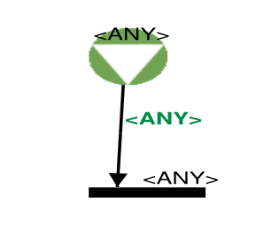
\includegraphics[scale=1.3]{ch3/img/xL2}}
 \quad{} \quad{}

\includegraphics{ch3/img/sep}
\quad{} \quad{}
\subfloat[RHS]{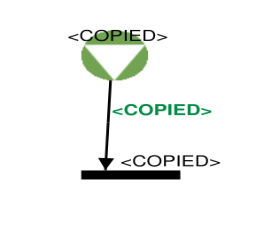
\includegraphics[scale=1.3]{ch3/img/xR2}}

\caption{\label{fig:edgotoraw}Edges from Raw Material into Operating unit to xml code} 

\end{figure} 
  
\paragraph{\emph{ a )~Condition for rule \ref{fig:edgotoraw} } } it is the same with figure \ref{fig:condition of Raw Material for Transfromation} but here we select the edges

\vspace{1cm} 
\begin{figure}[th]
	\centering  %[scale=1.2]
 	\includegraphics[scale=0.38]{ch3/img/xcond2}
	\caption{\label{fig:Condition2)}Condition of Edges ( RawMaterial to Operating unit)}
 \end{figure} 
\vspace{1cm}
\paragraph{\emph{ b )~Action for rule \ref{fig:edgotoraw} } }  we add this action to  Transform the Edges between Any Material and Any Operating unit into xml file, or to export the entitie from Graphical presentation 
into Xml Code  
\vspace{0.7cm}
\begin{figure}[th]
	\centering  %[scale=1.2]
 	\includegraphics[scale=0.38]{ch3/img/xact2}
	\caption{\label{fig:action2)}Action of Edges ( RawMaterial to Operating unit)}
\end{figure}  

and this code represent a Function to add new Edges into the Tree code 
to export the tree later 
 
\vspace{0.7cm}
\begin{lstlisting}[language=Python, caption=Python Function new Edges]
def newEdges(  parent, name, ID, xN, yN    ,beginID, endID    ):
	#Create new Node and add it into parent Node	
	node = ET.SubElement(parent, "Edge",ID=str(ID),BeginID=str(beginID),EndID=str(endID),Rate=str(name),Title=str(name), ArrowOnCenter="true", ArrowPosition="50")  
	#Create Corde for the node Edges
	cords = ET.SubElement(node, "Coords")
	ET.SubElement(cords, "X").text = str( xN )
	ET.SubElement(cords, "Y").text = str( yN )
	#Create Label for the Edges
	label = ET.SubElement(node, "Label",Text = str(name))
	offset = ET.SubElement(label,  "Offset")
	ET.SubElement(offset, "X").text =   str(5)
	ET.SubElement(offset, "Y").text =   str(0)
 
	return node 
\end{lstlisting}

% UPDATE 13.47

\pagebreak
\begin{itemize}
\item \textbf{Final Action :} it is to create the xml file instead after we generate the graph variable from previous rules  \ref{fig:Code Final Action}. 
   
\end{itemize}

\begin{figure}[th]
	\centering  %[scale=1.2]
 	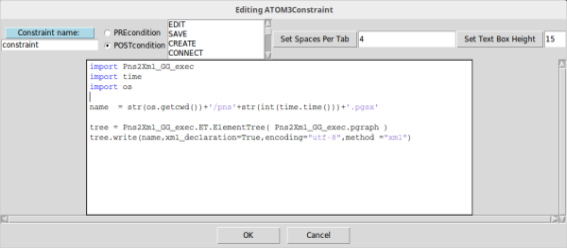
\includegraphics[scale=0.38]{ch3/img/FinAct}
	\caption{\label{fig:Code Final Action}Code Final Action}
\end{figure}
\section{Optimum structure of MaS \label{sec:optim} }

To optimize the multi-agent system in  Process Process synthesis, 
we choose a tool called  P-Graph Studio 

figure \ref{fig:Multi Agent System in PGraph Studio} represent multi agent system, Previously mentioned in figure \ref{fig:Complex Multi Agent System After transforamtion} 
\begin{figure}[th]
	\centering
		\includegraphics[scale=0.44]{ch3/img/pgraphArt}
	\caption{\label{fig:Multi Agent System in PGraph Studio}Multi Agent System in PGraph Studio}
\end{figure} 
\pagebreak
After we use this tool to optimise, we got this figure \ref{fig:Multi Agent System in Optimum structure}

\begin{figure}[th]
	\centering
		\includegraphics[scale=0.44]{ch3/img/pgraphSol}
	\caption{\label{fig:Multi Agent System in Optimum structure}Multi Agent System in Optimum structure}
\end{figure} 

PGraph Studio Generate 2 Files : 
\begin{itemize}
	\item Graph.in and contain :
		\begin{enumerate}
			\item information about Material, price, quanity
			\item information about operating unit, income material and outcome material 
 	\end{enumerate}

\end{itemize}

\begin{lstlisting}[caption=Part from Graph.in]
material-to_operating_unit_flow_rates:
A1_R1: A1 => 0.433 A1_R1_G1 + 0.433 A1_R1_G4 +
			 0.433 A1_R1_G3 + 0.433 A1_R1_G2
A1_R2: A1 => 0.433 A1_R2_G4 + 0.433 A1_R2_G3 + 
			 0.433 A1_R2_G2 + 0.433 A1_R2_G1
A2_R2: A2 => 0.633 A2_R2_G4 + 0.633 A2_R2_G3 + 
			 0.633 A2_R2_G2 + 0.633 A2_R2_G1
A3_R2: A3 => 0.5 A3_R2_G4 + 0.5 A3_R2_G3 + 
			 0.5 A3_R2_G2 + 0.5 A3_R2_G1
G1_OAF: G1 => OAF
G2_OAF: G2 => OAF
G3_OAF: G3 => OAF
G4_OAF: G4 => OAF

\end{lstlisting}


\section{Conclusion}
We have presented in this chapter  our approach of transformations of the MaS in OMACS framework to PNS, And we also presented our the 2nd
approach that transforms PNS Model into XML file after that we saw the tool PGraph Studio we use it to optimize multi agent system in pns frame work.

% 0200 kmiss
